\documentclass{article}

\usepackage{graphicx}
\usepackage{subfigure}
\usepackage[hypcap]{caption}
\usepackage{listings}
\usepackage{float}
\floatstyle{plaintop}
\restylefloat{table}

\title{Experimental Design and Data Analysis: Assignment 6}
\author{Andrew Bedard(2566978) \& Simone van Gompel(2567525) \\ Group 19}

\begin{document}

  \maketitle

  \section{Introduction}
    In this paper the process of analyzing a certain dataset is laid out.
    The dataset used is calcium.dat, which can be found at \url{http://www.amstat.org/publications/jse/jse_data_archive.htm}

  \section{The Experiment}

  \section{Data Analysis}
    First off a pairs plot was made of the data to be able to see how the data relates to each other.
    In Fig\ref{fig:FirstPairs} the foremost problem is clear, the outliers in the data are big and unlogical.
    Furthermore has Lab more than 6 categories, these problems can be explained by human error.
    And lastly the lab 3 has strange measurements with the cammol, this might be because of confusion of the measurement unit.
    The following values were changed:
    \begin{itemize}
      \item Removed Ages over 110
      \item Removed Sex which is not in the category 1 or 2
      \item Removed Lab categories which are over 6
      \item Removed Phosmmol over 2
      \item Divided Cammol of Lab 3 by 10 (this is visually tested by using a pairs plot)
    \end{itemize}
    After removal the same plot is made, see: Fig\ref{fig:SecondPairs}.
    Here you can see the correlations between the features better than in Fig\ref{fig:FirstPairs}.
    \begin{figure}[H]
        \centering
        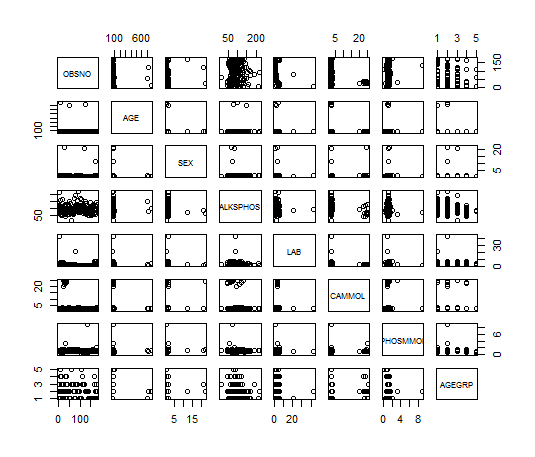
\includegraphics[scale=0.5]{../results/FirstPairs.png}
        \caption{Pairsplot of the original data}
        \label{fig:FirstPairs}
    \end{figure}
    \begin{figure}[H]
        \centering
        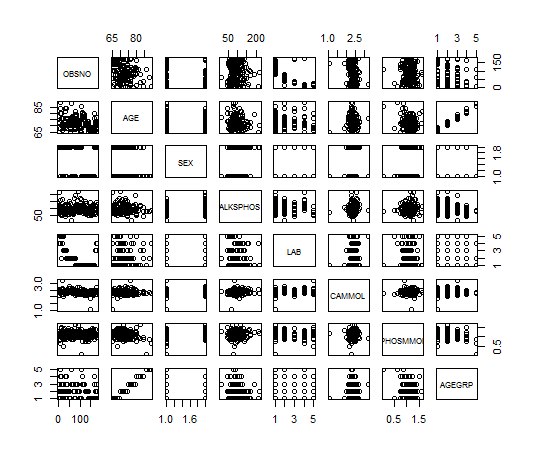
\includegraphics[scale=0.5]{../results/SecondPairs.png}
        \caption{Pairsplot of the updated data}
        \label{fig:SecondPairs}
    \end{figure}

  \section{Results}

  \section{Discussion}
    
  \section{R-Code}
    \begin{lstlisting}[language=R]
    \end{lstlisting}
\end{document}
